\documentclass[12pt,reqno]{article}

%%%%%%%%%%%%%%%%%%%% PACKAGES %%%%%%%%%%%%%%%%%%%%

\usepackage[utf8]{inputenc}
\usepackage[all]{xy}
\usepackage[T1]{fontenc}
\usepackage[usenames, dvipsnames]{color}
\usepackage{setspace}
\usepackage{dsfont}
\usepackage{amssymb}
\usepackage{amsthm,bbm}
\usepackage{amscd}
\usepackage{amsfonts}
\usepackage{stmaryrd}
\usepackage{amsmath}
\usepackage{graphicx}
\usepackage{multicol}
\usepackage{xspace}
\usepackage{extarrows}
\usepackage{color}
\usepackage [english]{babel}
\usepackage [autostyle, english = american]{csquotes}
\usepackage[colorlinks, linktocpage, citecolor = red, linkcolor = blue]{hyperref}
\usepackage{fullpage}
\usepackage{color}
\usepackage{euler}
\usepackage{parskip}
\usepackage{tikz}

%%%%%%%%%%%%%%%%%%%% INITIALIZATION %%%%%%%%%%%%%%%%%%%%

\MakeOuterQuote{"}
\graphicspath{ {./} }

%%%%%%%%%%%%%%%%%%%% COMMANDS %%%%%%%%%%%%%%%%%%%%

\newcommand{\range}{\mathrm{range\,}}
\newcommand{\nul}{\mathrm{null\,}}
\newcommand{\spn}{\mathrm{span\,}}
\newcommand{\card}{\mathrm{cardinality}}
\newcommand{\R}{\mathbb{R}}
\newcommand{\C}{\mathbb{C}}
\newcommand{\F}{\mathbb{F}}
\newcommand{\Z}{\mathbb{Z}}
\newcommand{\bd}{\mathrm{bd\,}}
\newcommand{\divline}{\hrule\vspace{12pt}\noindent}
\newcommand{\sgn}{\mathrm{sgn}}

%%%%%%%%%%%%%%%%%%%% ENVIRONMENTS %%%%%%%%%%%%%%%%%%%%

\theoremstyle{plain}
\newtheorem{maintheorem}{Theorem}
\renewcommand*{\themaintheorem}{\Alph{maintheorem}}

\newtheorem{theorem}{Theorem}[section] 
\newtheorem{lemma}{Lemma}
\newtheorem{corollary}[theorem]{Corollary}

\theoremstyle{definition}
\newtheorem{problem}{Problem}
\newtheorem{example}[theorem]{Example}
\newtheorem{definition}[theorem]{Definition}
\newtheorem{question}[theorem]{Question}

\newtheorem*{maintheorema}{Theorem \ref{thm:main}}

%%%%%%%%%%%%%%%%%%%% TITLE-PAGE %%%%%%%%%%%%%%%%%%%%

\title{MATH 1530 Problem Set 6}
\author{Tanish Makadia\\\small{(Collaborated with Esmé and Kazuya)}}
\date{March 2023}

%%%%%%%%%%%%%%%%%%%% DOCUMENT %%%%%%%%%%%%%%%%%%%%

\begin{document}
\maketitle

%%%%%%%%%%%%%%%%%%%% PROBLEM 1 %%%%%%%%%%%%%%%%%%%%

\begin{problem} 
    Let $G$ be a finite Abelian group and let $n$ be a positive integer that is relatively prime to $|G|$.
    Prove that the mapping 
    $a \mapsto a^n$
    is an automorphism of $G$.
\end{problem}

\begin{proof}
    Define \(\alpha : G\to G\) such that \(a\mapsto a^n\). Let \(g,h\in G\).
    \begin{enumerate}
        \item \textbf{Injective:} Suppose \(g^n=h^n\).
        \begin{align*}
            g^n=h^n &\implies e=g^nh^{-n}\\
            &\implies e=(gh^{-1})^n\\
            &\implies |gh^{-1}|\mid n
        \end{align*}
        Additionally, \(gh^{-1}\in G\). By \emph{Lagrange's Theorem}, we have \(|gh^{-1}|\mid |G|\).
        Since \(|gh^{-1}|\) divides both \(n\) and \(|G|\), and \(gcd(n, |G|)=1\), we have that \(|gh^{-1}|=1\).
        Therefore, \(gh^{-1}=e\implies g=eh\implies g=h\).

        \item \textbf{Surjective:} Consider \(g^n\). We have that \(g\mapsto g^n\).
        \item \textbf{Preserves Group Operation:} \(\alpha(gh)=(gh)^n=g^nh^n=\alpha(g)\cdot \alpha(h)\).
    \end{enumerate}
\end{proof}

\newpage
    
%%%%%%%%%%%%%%%%%%%% PROBLEM 2 %%%%%%%%%%%%%%%%%%%%

\begin{problem} 
    Let $G$ be a group of order $pqr$, where $p$, $q$, $r$ are distinct primes. If $H$ is a subgroup of $G$ of order $pq$ and $K$ is a subgroup of $G$ of order $qr$, prove that $|H \cap K| = q$.
\end{problem}

\begin{proof}
    We have already proven that \(H\cap K\) is a subgroup of \(G\). This implies that \(H\cap K\) is also a
    subgroup of \(H\) and \(K\). By \emph{Lagrange's Theorem}, we have that 
    \[|H\cap K|\mid |H|,|K|\implies |H\cap K|\mid pq,qr\]
    Therefore, \(|H\cap K|\) is either \(1\) or \(q\). Assume for contradiction that
    \(|H\cap K|=1\). By lemma \ref{lem:HK}, we have that
    \[|HK|=\frac{pq\cdot qr}{1}=pq^2r\]
    which is a contradiction since \(HK\) is a subset of \(G\), which implies that
    \(|HK|\leq|G|\). Therefore, we have shown that \(|H\cap K|=q\) as desired.
\end{proof}
\bigskip
\begin{lemma}
    \label{lem:HK}
    Let \(H\) and \(K\) be subgroups of a finite group \(G\). Then,
    \[|HK|=\frac{|H||K|}{|H\cap K|} \text{ where } HK=\{hk\ |\ h\in H,\ k\in K\}\]
    
    \begin{proof}
        We can separate \(HK\) into a union of left cosets of \(K\) in \(G\):
        \[HK=\bigcup_{h\in H} hK\]
        By the properties of cosets, we have that \(hK=h'K\) or \(hK\cap h'K=\emptyset\) for all
        \(h,h'\in H\). We must now determine how many of these cosets are distinct.
        
        Suppose \(hK=h'K\) for some \(h,h'\in H\). Since \(hK=h'K \Leftrightarrow h^{-1}h'\in K\), we have that
        \(h^{-1}h'=k\) for some \(k\in K\). This implies that \(k\in H\implies k\in H\cap K\).
        Additionally, \(h'=hk\). Thus, there are \(|H\cap K|\) ways to create the same coset for each \(h'\in H\)
        (by \emph{Cayley's Theorem}, we know that each \(k\in H\cap K\) has exactly one corresponding \(h\in H\) such that
        \(hk=h'\)). Therefore, the number of distinct cosets \(hK\) where \(h\in H\) is \(|H|/|H\cap K|\).

        Since \(|hK|=|h'K|\) for all \(h,h'\in H\), the number of elements in each coset is \(|hK|=|K|\). Therefore,
        the cardinality of \(HK\) equals the number of distinct cosets times the number of distinct elements in each coset, giving us
        \[|HK|=\frac{|H||K|}{|H\cap K|}\]
    \end{proof}
\end{lemma}

\newpage
    
%%%%%%%%%%%%%%%%%%%% PROBLEM 3 %%%%%%%%%%%%%%%%%%%%

\begin{problem} 
    Calculate the order of the group of rotations of a regular dodecahedron:
    \begin{center}
        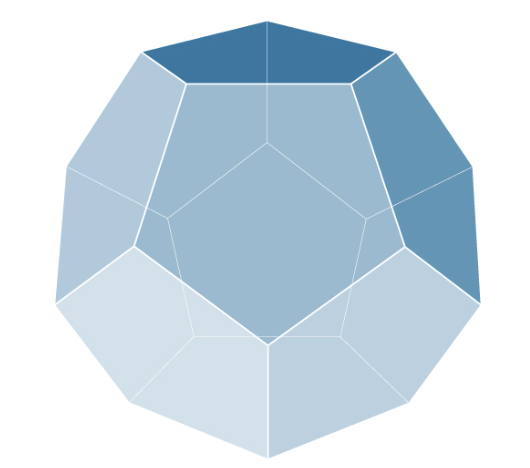
\includegraphics[height = 1.6 in]{Screenshot 2023-03-03 at 1.12.39 PM.png}
    \end{center}
\end{problem}

\begin{proof}
    Let \(G\) be the rotation group of the dodecahedron. Assign each of the 12 faces of the dodecahedron a unique number \(1-12\).
    Since every rotation must take each face to exactly one other face, \(G\) is a group of permutations
    on the set \(\{1,\ldots,12\}\). 
    
    Consider a single face, \(f\in\{1,\ldots,12\}\), of the dodecahedron.
    By the \emph{orbit-stabilizer theorem}, we have that 
    \[|G|=|orb_G(f)|\cdot |stab_G(f)|\]
    \begin{enumerate}
        \item \(\mathbf{|orb_G(f)|}:\) Picking an axis of rotation through the centers of any two
        parallel faces allows us to bring \(f\) to any other face \(f'\in\{1,\ldots,12\}\).
        Therefore, \(orb_G(f)=\{1,\ldots,12\}\) which implies that \(|orb_G(f)|=12\).
        \item \(\mathbf{|stab_G(f)|}:\) Let \(\overline{f}\in \{1,\ldots,12\}\) be the face parallel to \(f\). 
        Picking an axis of rotation through the centers of \(f\) and \(\overline{f}\) allows
        us to rotate the dodecahedron in \(5\) distinct ways while fixing the position of \(f\). 
        This implies that \(|stab_G(f)|=5\).
    \end{enumerate}
    Together, we have \(|G|=12\cdot 5=60\).
\end{proof}

\newpage
    
%%%%%%%%%%%%%%%%%%%% PROBLEM 4 %%%%%%%%%%%%%%%%%%%%

\begin{problem} 
    Determine the number of cyclic subgroups of order 15 in $\mathbb{Z}_{90} \oplus \mathbb{Z}_{36}$.
\end{problem}

\begin{proof}
    A cyclic subgroup of order \(15\) has \(\phi(15)=8\) distinct elements of order \(15\).
    We will now determine the number of distinct elements of order \(15\) in \(\Z_{90}\oplus\Z_{36}\).
    
    Let \((g_1,g_2)\in\Z_{90}\oplus\Z_{36}\) such that \(|(g_1,g_2)|=15\).
    By \emph{(Gallian, Theorem 8.1)}, we have that \(lcm(|g_1|,|g_2|)=15\).
    For each of the resulting cases, we can use the \emph{Euler phi function} since \(\Z_{90}\) and
    \(\Z_{36}\) are both cyclic.
    \begin{enumerate}
        \item \textbf{(\(\mathbf{|g_1|=5,\ |g_2|=3}\)):} 
            \begin{itemize}
                \item \(\phi(5)=4\implies 4\) distinct elements of order
                \(5\) in \(\Z_{90}\).
                \item \(\phi(3)=2\implies 2\) distinct elements of order \(3\) in \(\Z_{36}\).
            \end{itemize}
            Therefore, we have \(4\cdot 2=8\) ways to make \((g_1,g_2)\) from this case.
        
        \item \textbf{(\(\mathbf{|g_1|=15,\ |g_2|=1}\)):} 
            \begin{itemize}
                \item \(\phi(15)=8\implies 8\) distinct elements of order
                \(15\) in \(\Z_{90}\).
                \item \(\phi(1)=1\implies 1\) distinct element of order \(1\) in \(\Z_{36}\).
            \end{itemize}
            So there are \(8\cdot 1=8\) ways to make \((g_1,g_2)\) from this case.
        
        \item \textbf{(\(\mathbf{|g_1|=15,\ |g_2|=3}\)):} 
            From above, we have \(8\) distinct elements of order
            \(15\) in \(\Z_{90}\), and \(2\) distinct elements of order \(3\) in \(\Z_{36}\).
            Hence, there are \(8\cdot 2=16\) ways to make \((g_1,g_2)\) from this case.
    \end{enumerate}
    In total, there are \(8+8+16=32\) distinct elements of order \(15\) in \(\Z_{90}\oplus\Z_{36}\). Since
    each cyclic subgroup of order \(15\) is disjoint and has \(8\) distinct elements of order \(15\)
    which can generate it, the number of cyclic subgroups of order \(15\) in \(\Z_{90}\oplus\Z_{36}\) is \(32/8=4\).
\end{proof}

\newpage
    
%%%%%%%%%%%%%%%%%%%% PROBLEM 5 %%%%%%%%%%%%%%%%%%%%

\begin{problem} 
    Let $p$ and $q$ be odd primes and let $m$ and $n$ be positive integers. Prove that $U(p^m) \oplus U(q^n)$ is not cyclic. [hint: read the book to find a useful result we didn't cover in class]
\end{problem}

\begin{proof}
    By \emph{(Gallian, pg. 160)}, we have that \(U(p^m)\approx\Z_{p^m-p^{m-1}}\) and \(U(q^n)\approx\Z_{q^n-q^{n-1}}\). 
    Because \(\Z_{p^m-p^{m-1}}\) and \(\Z_{q^n-q^{n-1}}\) are both cyclic, we have that \(U(p^m)\) and \(U(q^n)\) are cyclic
    as well. Therefore, by \emph{(Gallian, Theorem 8.2)}, we must show that \(|U(p^m)|\) and \(|U(q^n)|\)
    are not relatively prime.

    By lemma \ref{lem:phi}, we have that \(|U(p^m)|=p^m-p^{m-1}\) and \(|U(q^n)|=q^n-q^{n-1}\). Since the product of odds is odd,
    \(p^m\), \(p^{m-1}\), \(q^n\), and \(q^{n-1}\) must all be odd. Since the difference of odds is even, we have that
    \(2\mid p^m-p^{m-1},q^n-q^{n-1}\implies gcd(p^m-p^{m-1},q^n-q^{n-1})\neq 1\). Therefore, \(|U(p^m)|\) and \(|U(q^n)|\) are not
    relatively prime, which means \(|U(p^m)|\oplus|U(q^n)|\) is not cyclic.
\end{proof}

\newpage

\begin{lemma}
    \label{lem:iso}
    Let \(p\) be an odd prime. Then \(U(p^n)\approx \Z_{p^n-p^{n-1}}\).
    \begin{proof}
        By lemma \ref{lem:phi}, we have that \(|U(p^n)|=p^n-p^{n-1}\). We can arrange the elements of \(U(p^n)\) in ascending order
        so that \(U(p^n)=\{u_1,\ldots,u_{p^n-p^{n-1}}\}\) where \(j<k\implies u_j<u_k\). Similarly, we can arrange the
        elements of \(\Z_{p^n-p^{n-1}}\) in ascending order so that \(\Z_{p^n-p^{n-1}}=\{z_1,\ldots,z_{p^n-p^{n-1}}\}\) where
        \(j<k\implies z_j<z_k\).

        Define a mapping \(\phi: U(p^n)\to \Z_{p^n-p^{n-1}}\) such that \(u_i\mapsto z_i\). We will now show that
        \(\phi\) is an isomorphism. Let \(z_m,z_n\in\Z_{p^n-p^{n-1}}\).
        \begin{enumerate}
            \item \textbf{Injective:} to be proved \(\ldots\)
            \item \textbf{Surjective:} to be proved \(\ldots\)
            \item \textbf{Preserves Group Operation:} \(\phi(u_m\cdot u_n)=\phi((u_mu_n))= \ldots\) to be proved
        \end{enumerate}
    \end{proof}
\end{lemma}

\bigskip

\begin{lemma}
    \label{lem:phi}
    Let \(p\) be an odd prime. Then \(\phi(p^n)=p^n-p^{n-1}\).
    \begin{proof}
        We will show \(|U(p^n)|=p^n-p^{n-1}\). Of course, there are \(p^n\) integers up to \(p^n\). Therefore,
        \(|U(p^n)|=p^n-m\) where \(m\) is the number of integers in the set \(\{1,\ldots,p^n\}\) 
        that are not relatively prime with \(p^n\). Evidently, the prime factorization of \(p^n\) only contains
        the prime \(p\). This implies that \(p\) divides every integer that is not relatively prime with \(p^n\).
        The number of such integers in the set \(\{1,\ldots,p^n\}\) is \(p^n/p\). Therefore,
        \[|U(p^n)|=p^n-m=p^n-\frac{p^n}{p}=p^n-p^{n-1}\]
    \end{proof}
\end{lemma}

\end{document}